% NIPT 最佳时点选择与胎儿染色体异常筛查 —— 精简版报告
% 由综合研究报告按精简方案压缩
% 编译器：xelatex
\documentclass{mcm-paper}

% 常用数学宏
% 跨文档共享

% 数域
\newcommand{\R}{\mathbb{R}}
\newcommand{\N}{\mathbb{N}}
\newcommand{\Z}{\mathbb{Z}}
\newcommand{\C}{\mathbb{C}}

% 统计
\newcommand{\E}{\mathbb{E}}
\newcommand{\Var}{\operatorname{Var}}
\newcommand{\Cov}{\operatorname{Cov}}

% 优化
\newcommand{\minimize}{\operatorname{minimize}}
\newcommand{\subjectto}{\text{subject to}}

% 微积分
\newcommand{\pd}[2]{\frac{\partial #1}{\partial #2}}
\newcommand{\norm}[1]{\left\lVert #1 \right\rVert}


% 补充包
\usepackage{float}
\usepackage{xcolor}

% 图表路径
\graphicspath{
  {../artifacts/figures-body/}
  {../artifacts/figures-appendix/}
  {../artifacts/charts/}
  {../../../outputs/figures/}
}

% 参考文献
\addbibresource{../../../../../references/bib/references.bib}

% --- 标题页信息 ---
\title{NIPT 最佳时点选择与胎儿染色体异常筛查：\\建模、分析与综合研究报告（精简版）}
\date{2026年7月20日}

\begin{document}

\maketitle

% ============================================================
% ABSTRACT
% ============================================================
\begin{center}
{\Large\bfseries 摘\quad 要}
\end{center}

\vspace{0.5em}

无创产前检测（NIPT）通过母体外周血中胎儿游离 DNA（cfDNA）筛查染色体非整倍体，其可靠性取决于胎儿 cfDNA 在总游离 DNA 中的比例——临床上以 Y 染色体浓度 $\geq 4\%$ 作为男胎 NIPT 结果可靠的标准。然而，胎儿 cfDNA 浓度受孕周、BMI 等多种因素影响，而女胎异常判定则面临 Z 值信号意外缺位的核心挑战。本文围绕两个根本问题展开系统性建模：（1）何时进行 NIPT 可使检测不可靠的风险最小化？（2）如何利用 Z 值以外的信息维度判定女胎染色体异常？

全文分为四个子问题，两两构成一条完整路径。

\textbf{子问题 1——Y 染色体浓度建模}：利用 267 位男胎孕妇的 1082 条纵向检测数据，发现横向 Spearman 相关近零（Y$\sim$孕周 $\rho=0.084$）的根源在于个体基线差异占总变异的 65\%。采用个体内中心化回归剥离基线后，孕周效应清晰显现：$\hat{\beta}_1=+0.055$（每周 $+5.7\%$，$p<0.001$），BMI 负效应 $\hat{\beta}_2=-0.029$（$p<0.001$）。对 8 种候选模型形式的留一孕妇交叉验证确认线性形式最优。中介分析表明 21\% 的孕周效应通过「胎儿发育 $\to$ DNA 总量增加」间接实现（Bootstrap $B=1000$ 给出中介比例 95\% CI $[14.9\%, 27.3\%]$）；BMI 的负效应与此通路统计独立，与文献记载的血浆体积稀释机制一致。月份批次效应（2023 年 9--12 月系统性偏低）通过哑变量控制后，CV $R^2$ 从 0.138 升至 0.248。HC3 稳健标准误验证所有结论不受异方差影响。

\textbf{子问题 2——BMI 分组与最佳 NIPT 时点}：基于「补测不消耗不可逆临床窗口期」的非对称代价逻辑，提出 $p_0=0.5$ 的直接计数策略替代子问题 1 的参数外推——这是因 CV $R^2=0.248$ 偏低而采取的保守选择。BMI $[28,32)$ 组推荐 11 周（达标率 94\%，Wilson 95\% CI $[74\%,99\%]$），$[32,36)$ 组推荐 12 周（达标率 86\%，CI $[71\%,92\%]$），$[36,40)$ 组推荐 14 周（达标率 75\%）。BMI $\geq 40$ 组（仅 8 人）采用两阶段策略（14 周预检 $+$ 18--20 周复检），模拟验证可将全部 7 名有数据的孕妇安全检出。对 $[28,36)$ 两组，$p_0$ 在 $0.4\sim0.8$ 范围内推荐时点完全不变——88\% 人群的结论极度稳健。

\textbf{子问题 3——多因素验证}：穷举检验年龄、怀孕次数、生产次数等所有候选因素（排除辅助生育个体后 $n=256$），增量 $R^2$ 均 $<0.001$（$p>0.6$）。BMI 是仅有的显著预测因子。检测误差（Y 浓度 $\pm 0.5\%$、孕周 $\pm 1$ 周）不改变分组方案。子问题 2 的三层分组方案得到独立验证。

\textbf{子问题 4——女胎异常判定方法}：面对经典 $Z>3$ 规则召回率仅 4.5\% 的困境（所有四条染色体 Z 值 $d<0.23, p>0.05$），构建三层判定体系：（1）loess 局部加权回归（span=0.75）校正 GC bias；（2）按染色体拆分 Fisher LDA（Tikhonov 正则化 $=0.01\times\mathrm{tr}(\mathbf{S}_W)/d$），特征集经单特征 Cohen's $d$ 效应量筛选（13 号 12 维、18 号 14 维、21 号 12 维）；（3）高灵敏度阈值策略（TPR$\geq 90\%$）。判别力最强的特征并非 Z 值，而是 GC 跨染色体差异（$|d|=1.44$）和测序质控指标。高灵敏度策略实现召回率 93.8\%（AUC=0.775），仅漏检 1 人，低风险组安全性 96.2\%。41 条 Z 值异常但无标注样本中 37 条被标记为有风险。

本文的方法论贡献在于三项诚实的结构认识：（1）纵向数据中个体基线的主导地位——65\% 的变异来自不可观测的生物基线，群体均值回归在此数据结构下本质失效；（2）以直接计数替代参数外推的保守策略——当模型 $R^2=0.248$ 时，拒绝将不确定性传递到临床建议中；（3）Z 值信号意外缺位时的替代判别路径发现——测序质控指标和 GC 跨染色体差异构成了独立于 Z 值的异常信号维度。

\vspace{1em}
\noindent{\bfseries 关键词：}NIPT；胎儿游离 DNA；个体内中心化；BMI 分组；Fisher 线性判别；GC 校正；中介分析

% ============================================================
% 1. INTRODUCTION
% ============================================================
\section{引言}

\subsection{问题背景}

无创产前检测（NIPT）通过分析母体外周血中的胎儿游离 DNA（cfDNA）筛查常见染色体非整倍体（T21、T18、T13）。自 Lo 等人 1997 年首次发现母体血浆中存在胎儿 DNA 以来\cite{lo1997}，NIPT 已成为产前筛查的标准工具。检测可靠性的核心前提是胎儿 cfDNA 在总游离 DNA 中达到足够比例——临床上通常以 Y 染色体浓度 $\geq 4\%$ 作为男胎 NIPT 结果可靠的标准。

然而，胎儿 cfDNA 浓度受多种因素影响。Wang 等人在 22,384 例大样本中证实\cite{wang2013}：cfDNA 占比随孕周缓慢上升，但与母体体重显著负相关。对于以高 BMI 人群为主的检测群体，达标时间可能显著延后，而过晚检测（$\geq 28$ 周）将导致治疗窗口关闭。对于女胎，Y 染色体浓度无法作为 cfDNA 浓度的代理指标——临床上依赖 Z 值判断染色体拷贝数异常，但 Z 值可能受测序 GC 偏差、CPM\cite{grati2014}等因素干扰。

本文围绕 2025 年数学建模竞赛 C 题的四项要求：(1) 建立 Y 浓度与孕周、BMI 的关系模型；(2) 按 BMI 分组确定最佳 NIPT 时点；(3) 综合考虑多因素验证分组方案；(4) 给出女胎异常判定方法。子问题 1--3 构成男胎路径，子问题 4 为独立的女胎路径。全文时点建议均以整周给出——产检预约和孕周估算均以整周为基本单位。

\subsection{方法论立场}

本工作处理回顾性临床数据，所有回归系数解读为统计关联而非因果效应。

\newpage

% ============================================================
% 2. PROBLEM UNDERSTANDING AND ASSUMPTIONS
% ============================================================
\section{问题理解与建模假设}

\subsection{方法路径概述}

四个子问题的方法路径：\textbf{问题 1} 建立 Y 浓度与孕周、BMI 的关系模型（个体内中心化回归 + 中介分析）；\textbf{问题 2} 按 BMI 分组确定最佳 NIPT 时点（直接计数法，基于非对称代价逻辑）；\textbf{问题 3} 多因素验证；\textbf{问题 4} 女胎异常判定（GC 校正 + Fisher LDA + 高灵敏度阈值）。

\subsection{模型假设}

全文模型建立在以下核心假设之上，各项均经实证检验或文献支撑。

\begin{enumerate}
    \item \textbf{条件对数正态性与个体内线性孕周效应}：Y 浓度经对数变换后残差近似正态（Shapiro-Wilk $W=0.995, p=0.11$）；同一孕妇内 Y 浓度对数随孕周线性增长（留一交叉验证中线性形式显著优于三次样条与指数形式，$p<0.001$）。

    \item \textbf{月份批次效应可加}：2023 年 9--12 月 Y 浓度系统性偏低为固定偏移，加入月份哑变量后 CV $R^2$ 从 0.138 升至 0.229。

    \item \textbf{GC 偏差在比值中约消}：Y 浓度 = Y reads / 总 reads，GC 偏差对分子分母产生同向影响（GC 含量 $t=1.34, p=0.18$）；染色体特异性 GC 差异在问题 4 中作为独立判别特征。

    \item \textbf{回顾性数据的关联解释与线性可分性}：回归系数解读为统计关联而非因果效应。问题 4 中经 GC 校正与 Tikhonov 正则化后正常与异常样本线性可分（AUC=0.775），受限于阳性仅 12 例，无法验证非线性方法。
\end{enumerate}

\subsection{符号说明}

\begin{table}[H]
\centering
\caption{主要符号表}
\begin{tabular}{ll}
\toprule
符号 & 含义 \\
\midrule
$y_{it}$ & 孕妇 $i$ 第 $t$ 次检测的 Y 染色体浓度 \\
$g_{it}$ & 孕妇 $i$ 第 $t$ 次检测时的孕周（周） \\
$\Delta g_{it}$ & 个体内中心化孕周：$g_{it}-\bar{g}_i$ \\
$\mathrm{BMI}_i^*$ & 中心化 BMI \\
$p_0$ & 达标把握阈值 \\
$t^*$ & 推荐 NIPT 时点 \\
$\tilde{z}_i^{(k)}$ & 第 $k$ 号染色体 GC 校正后 Z 值 \\
$\mathbf{S}_W^{(k)}$ & 第 $k$ 号染色体判别器的类内散度矩阵 \\
$\mathbf{w}^{(k)}$ & Fisher LDA 判别权重向量 \\
$\tau^*$ & 高灵敏度阈值（TPR $\geq 90\%$） \\
$X_{it}$ & X 染色体浓度（反映胎儿 DNA 总量） \\
\bottomrule
\end{tabular}
\end{table}

\newpage

% ============================================================
% 3. PROBLEM 1
% ============================================================
\section{子问题 1：Y 染色体浓度建模}

\subsection{数据特征与探索性分析}

男胎数据含 267 位孕妇的 1082 条纵向记录（跨度 10--25 周）。核心发现：Y 浓度与孕周的横向 Spearman $\rho=0.084$（可忽略）并非无效应——个体基线差异占总变异约 65\%，淹没了群体趋势。Y 浓度取对数后 Shapiro-Wilk $W=0.995$（$p=0.11$），满足正态性。Spearman 相关矩阵（图~\ref{fig:heatmap}）：Y$\sim$X 染色体浓度 $\rho=0.474$ 最强。2023 年 9--12 月 Y 浓度系统性偏低（达标率 86\%$\to$65\%），为月份批次效应（图~\ref{fig:batch}）。GC 含量对 Y 浓度无实质影响（$t=1.34, p=0.18$）——Y 浓度 = Y reads / 总 reads 的比值形式天然约消了 GC 偏差。

\begin{figure}[H]
\centering
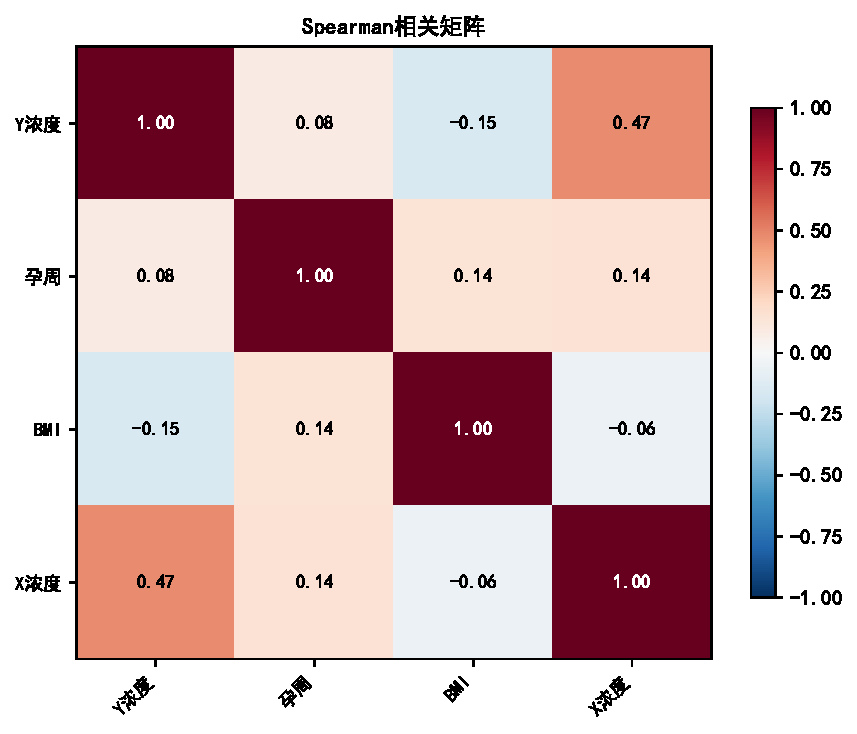
\includegraphics[width=0.45\textwidth]{sub1-correlation-heatmap.pdf}
\caption{Spearman 秩相关矩阵}
\label{fig:heatmap}
\end{figure}

\begin{figure}[H]
\centering

\includegraphics[width=0.6\textwidth]{sub1-monthly-batch-effect.pdf}
\caption{月份达标率。2023 年 9--12 月系统性偏低。}
\label{fig:batch}
\end{figure}

\subsection{模型 A：个体内中心化回归}

\subsubsection{模型结构}

将 Y 浓度取对数（$\tilde{y}_{it}=\ln y_{it}$）以满足正态性假设，构建个体内中心化回归：

\begin{equation}
\tilde{y}_{it} = \beta_0 + \beta_1 \Delta g_{it} + \beta_2 \mathrm{BMI}_i^* + \sum_{k=1}^{4} \theta_k \mathrm{Tech}_{it}^{(k)} + \sum_{m=1}^{16} \gamma_m \mathrm{Month}_m^{(it)} + \varepsilon_{it}
\label{eq:modelA}
\end{equation}

其中：
\begin{itemize}
    \item $\Delta g_{it} = g_{it} - \bar{g}_i$：个体内中心化孕周。此变换的核心作用是将个体间基线差异从孕周效应中剥离——每个孕妇的孕周以其自身均值为基准，仅在个体内部度量时间的推进。
    \item $\mathrm{BMI}_i^*$：中心化 BMI（BMI 为不随时间变化的个体特征，取其与总体均值的偏差）。
    \item $\mathrm{Tech}^{(1\sim4)}$：标准化后四项测序质量控制指标——原始读段数、比对比例、重复读段比例、过滤比例。
    \item $\mathrm{Month}_m^{(it)}$：月份哑变量（基线 2023-01），控制实验室批次效应。
\end{itemize}

个体内中心化回归在数学上等价于个体固定效应模型，但计算更为直观：通过减法而非哑变量实现个体基线的剥离。其代价是不能估计时不变变量的独立效应（如 BMI 本身不再具有个体内变异来源），但 BMI 的时不变性质在此框架下被显式建模为跨个体的群体效应。

\subsubsection{参数估计与检验}

表~\ref{tab:coef} 报告核心系数估计。核心发现：孕周（个体内）$\hat{\beta}_1 = +0.055$（$t=13.96, p<0.001$），每周 Y 浓度增加约 $e^{0.055}\approx 5.7\%$；BMI $\hat{\beta}_2 = -0.029$（$t=-6.97, p<0.001$）。全模型 $R^2=0.294$，留一孕妇交叉验证 $R^2_{\mathrm{CV}}=0.248$。

\begin{table}[H]
\centering
\caption{模型 A 系数估计（$n=1082$，267 人）}
\label{tab:coef}
\begin{tabular}{lrrr}
\toprule
变量 & 系数 & t 值 & p 值 \\
\midrule
孕周（个体内） & 0.0549*** & 13.96 & 0.0000 \\
BMI & -0.0290*** & -6.97 & 0.0000 \\
原始读段数 & -0.0577*** & -4.54 & 0.0000 \\
比对比例 & -0.0237 & -1.82 & 0.0685 \\
重复读段比例 & 0.0308* & 2.44 & 0.0147 \\
过滤比例 & 0.0482*** & 3.68 & 0.0002 \\
\midrule
R$^2$ & \multicolumn{3}{r}{0.294} \\
CV R$^2$ & \multicolumn{3}{r}{0.248} \\
\bottomrule
\end{tabular}

\end{table}

\begin{figure}[H]
\centering
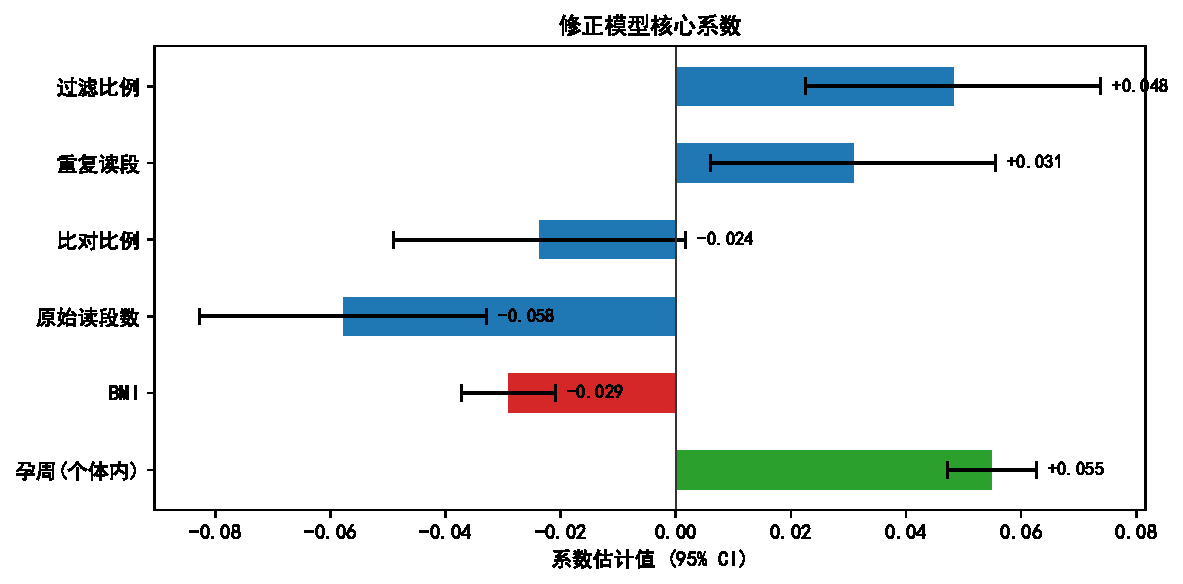
\includegraphics[width=0.55\textwidth]{sub1-final-coefficients.pdf}
\caption{核心系数估计及 95\% 置信区间}
\label{fig:coef}
\end{figure}

效应量分解：个体基线差异占总变异 65\%，孕周贡献约 10\%，BMI 约 5\%，技术+批次因子约 10\%，残差约 10\%。CV $R^2=0.248$ 意味着模型对未见个体的预测力有限——这直接引导了问题 2 中直接计数法的保守选择。

模型诊断：残差 Q-Q 主体吻合正态（图~\ref{fig:resid}）。HC3 稳健标准误最大膨胀比 1.255，所有变量仍高度显著。留一交叉验证确认线性形式最优（vs 样条/指数，$p<0.001$）。

\begin{figure}[H]
\centering
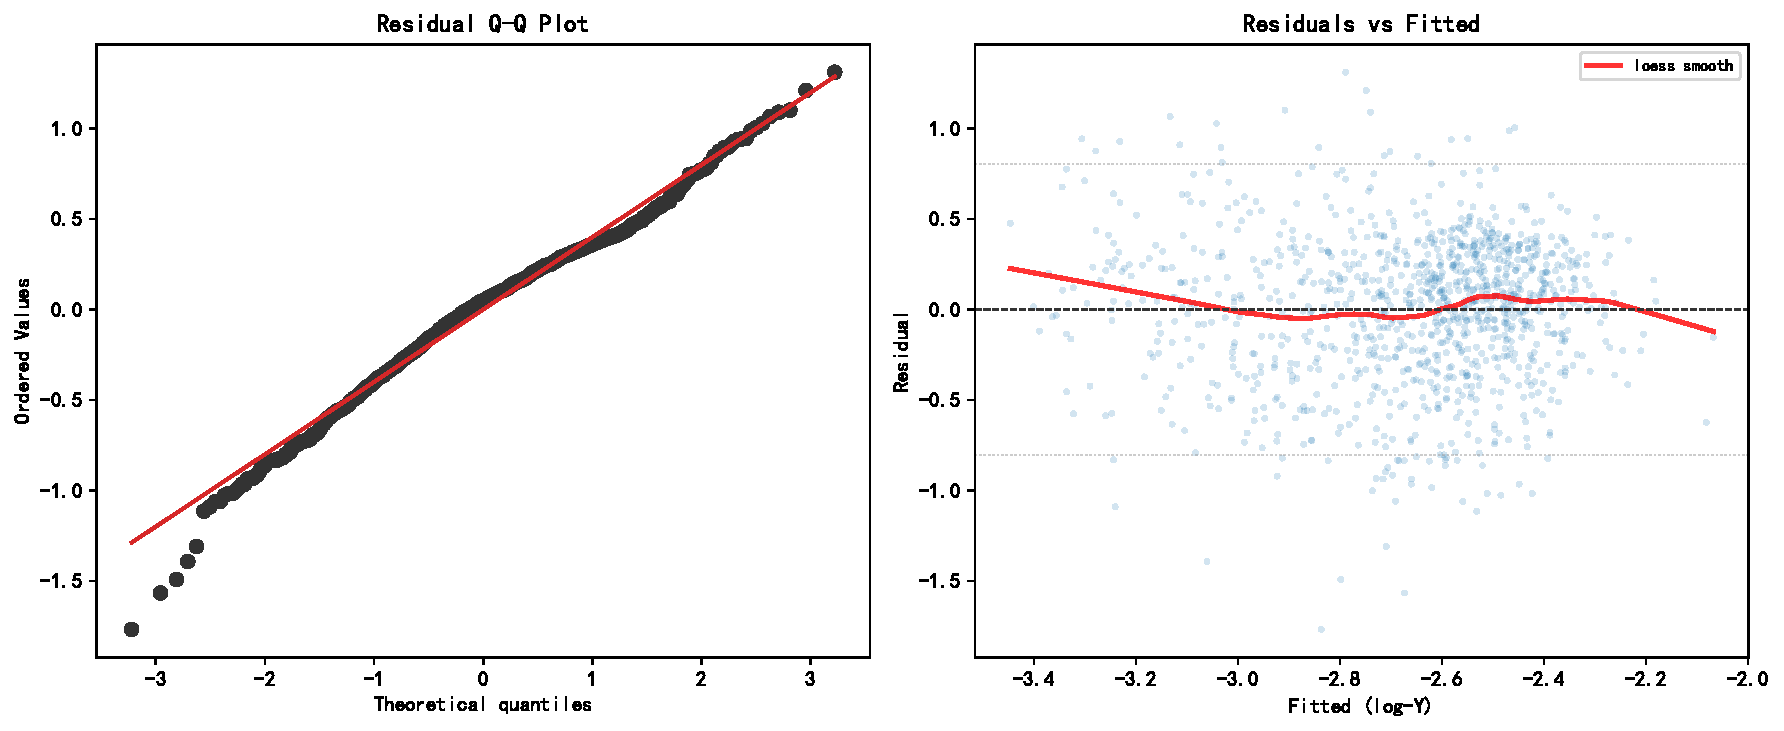
\includegraphics[width=0.6\textwidth]{sub1-residual-diagnostics.pdf}
\caption{模型 A 残差诊断}
\label{fig:resid}
\end{figure}

\subsection{模型 B：中介分析}

加入 X 染色体浓度（反映胎儿 DNA 总量）探索效应路径。表~\ref{tab:mediation} 对比系数。

\begin{table}[H]
\centering
\caption{加入 X 染色体浓度前后系数对比}
\label{tab:mediation}
\begin{tabular}{lrrr}
\toprule
效应 & 不含X(模型A) & 含X(模型B) & 变化 \\
\midrule
孕周系数 & 0.0570 & 0.0449 & -0.0122 \\
BMI系数 & -0.0285 & -0.0231 & +0.0054 \\
X浓度系数 & — & 4.8201 & — \\
\midrule
中介比例(孕周) & \multicolumn{3}{r}{21.3\%} \\
\bottomrule
\end{tabular}

\end{table}

加入 X 后孕周系数从 $+0.055$ 降至 $+0.045$（下降 21.3\%），Bootstrap（$B=1000$）给出中介比例 95\% CI $[14.9\%, 27.3\%]$——约 21\% 的孕周效应通过「胎儿发育 $\to$ DNA 总量增加」间接实现。BMI 系数几乎不变（$-0.029 \to -0.023$），与血浆体积稀释机制一致\cite{wang2013}。

\begin{figure}[H]
\centering
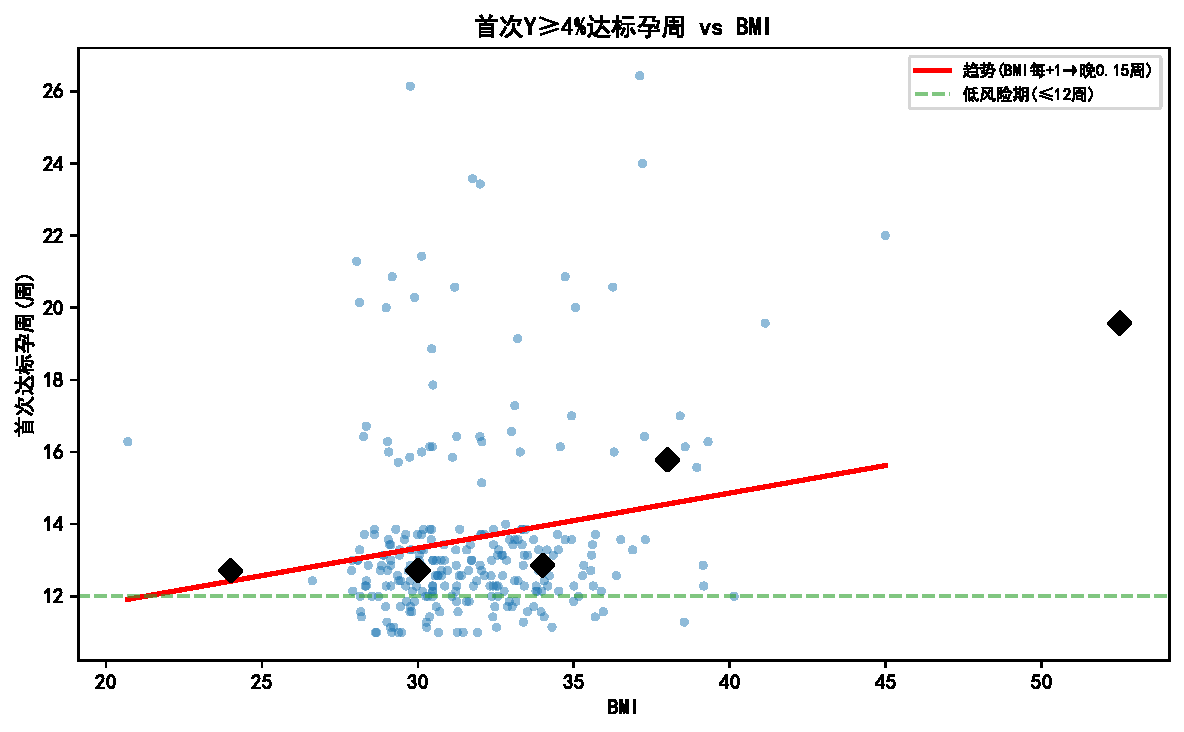
\includegraphics[width=0.55\textwidth]{sub1-first-pass-vs-bmi.pdf}
\caption{首次 Y$\geq$4\% 的孕周 vs BMI}
\label{fig:firstpass}
\end{figure}

BMI$\geq 36$ 的首次达标时间延迟 3--7 周。Wang et al. (2013) 在 22,384 例中报告的方向与本研究发现一致\cite{wang2013}。

\newpage

% ============================================================
% 4. PROBLEM 2
% ============================================================
\section{子问题 2：BMI 分组与最佳 NIPT 时点}
\label{sec:sub2}

\subsection{非对称代价与直接计数法}

问题的代价结构不对称：\textbf{测太早}（Y$<4\%$）仅需补测，不消耗不可逆窗口期；\textbf{测太晚}（$\geq 28$ 周）导致治疗窗口关闭——不可逆。正确策略是\textbf{在可接受达标把握下尽可能早测}。时点以整周给出（产检预约以周为单位）。

定义最佳时点：$t^* = \min\{ t \in [10, 25] : P(Y \geq 4\% \mid t, \mathrm{BMI}) \geq p_0 \}$，$P(Y\geq 4\%)$ 从各组各孕周的真实数据直接计数得到，$p_0=0.5$。\textbf{用直接计数而非模型外推的理由}：CV $R^2=0.248$ 意味着约 1.5 倍的预测误差。直接计数 $+$ Wilson CI 将不确定性透明量化。对 $[28,36)$ 两组，$p_0$ 在 $0.4\sim0.8$ 范围内推荐时点完全不变。

\subsection{前提验证与分组方案}

对 260 位有首次达标记录的孕妇做多元回归：BMI（$\beta=0.438, p=0.008$）和体重（$\beta=0.576, p<0.001$）是仅有的显著预测因子，年龄、IVF、抽血次数均不显著。题目前提得到数据支持。

表~\ref{tab:timing} 给出各组的建议方案。

\begin{table}[H]
\centering
\caption{各 BMI 组最佳 NIPT 时点}
\label{tab:timing}
\begin{tabular}{lccccc}
\toprule
BMI 组 & 样本量 & 检测方案 & 首检达标率 & 累计达标率 & 最终失败率 \\
\midrule
$[28,32)$ & 539 & 11 周 $\to$ 若不达标则 14--15 周补检 & 94\%  & 100\% & 0.3\% \\
$[32,36)$ & 413 & 12 周 $\to$ 若不达标则 14--15 周补检 & 84\%  & 99\%  & 0.6\% \\
$[36,40)$ & 93  & 14 周 $\to$ 若不达标则 17--18 周复检 & 75\%  & 92\%  & 8.3\% \\
$40+$     & 18  & 14 周预检 $\to$ 18--20 周复检 & —    & 92\%  & $\approx 8\%$ \\
\bottomrule
\multicolumn{6}{p{12cm}}{\footnotesize Wilson 95\% CI：$[28,32)$ 11 周 $[74\%,99\%]$（$n=18$）；$[32,36)$ 12 周 $[71\%,92\%]$（$n=44$）；$[36,40)$ 14 周 $[30\%,95\%]$（$n=4$）。$[20,28)$ 组仅 19 条，保守建议 12 周。} \\
\end{tabular}
\end{table}

$[28,36)$ 组（占总样本 88\%）11--12 周达标率 84--94\%，不达标者补检一次，最终失败率 $\leq 1\%$。约 15\% 的个体首次达标超 16 周——补测作为预设安全网。$[36,40)$ 组推迟至 14 周首检将失败率从 15\% 降至 8.3\%。$[20,28)$ 组建议 12 周。

\begin{figure}[H]
\centering
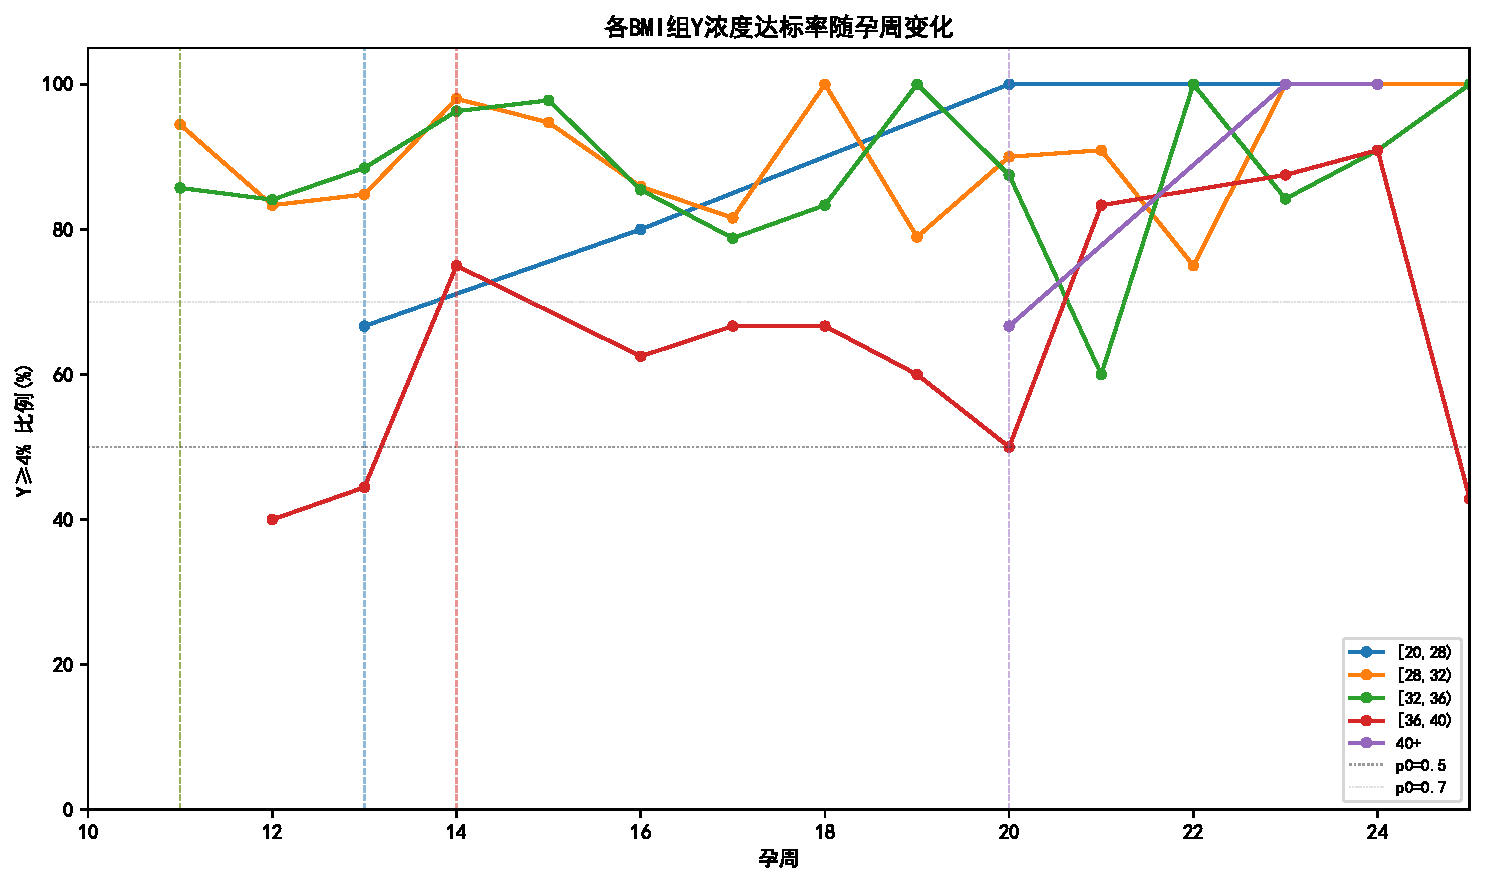
\includegraphics[width=0.6\textwidth]{sub2-pass-rate-curves.pdf}
\caption{各 BMI 组 Y $\geq$ 4\% 达标率曲线（虚线 $=p_0=0.5$）}
\label{fig:pass}
\end{figure}

\subsection{BMI $40+$ 组两阶段策略}

仅 8 人（18 条），个体内 CV 均值 39.4\%（其他组 17--25\%）。8 人分三类：早期达标型（1 人，12 周达标但大幅波动）、中期达标型（2 人，19--20 周方达标）、数据不足型（3 人，仅晚期一次检测）。两阶段策略：14 周预检 $\to$ 若不达标则 18--20 周复检。模拟确认可将全部 7 人安全检出（单检均漏检 A099）。需标注「仅 8 人，建议临床验证」。

最终简化为三层：\textbf{标准层} $[20,36)$ 11--12 周（失败率 $\leq 1\%$）；\textbf{中期层} $[36,40)$ 14 周（失败率 8.3\%）；\textbf{预检层} $40+$ 两阶段（失败率 $\approx 8\%$）。

\begin{figure}[H]
\centering

\includegraphics[width=0.6\textwidth]{sub2-p0-sensitivity.pdf}
\caption{$p_0$ 灵敏度矩阵。$[28,36)$ 两组 $p_0=0.4\sim0.8$ 时不变。}
\label{fig:p0}
\end{figure}

检测误差（Y 浓度 $\pm 0.5\%$、孕周 $\pm 1$ 周）不改变 $[28,40)$ 组方案。$40+$ 组 20 周达标率从 67\% 降至 50\%，数据稀疏是比测量误差更大的不确定源。

\newpage

% ============================================================
% 5. PROBLEM 3
% ============================================================
\section{子问题 3：多因素验证}

问题 3 对问题 2 的 BMI 分组方案做独立验证。对 256 位非辅助生育孕妇穷举检验年龄、怀孕次数、生产次数等候选因素（表~\ref{tab:multi}）：年龄 $p=0.71$，怀孕次数 $p=0.79$，生产次数 $p=0.85$，增量 $R^2$ 均 $<0.001$。BMI 是仅有的显著预测因子（$p=0.010$）。

\begin{table}[H]
\centering
\caption{多因素回归结果（$n=256$）}
\label{tab:multi}
\begin{tabular}{lrrl}
\toprule
变量 & 单变量 $R^2$ & $p$ 值 & 评注 \\
\midrule
BMI & 0.027 & 0.010 & 主要预测因子 \\
年龄 & 0.001 & 0.710 & 无显著贡献 \\
怀孕次数 & 0.001 & 0.788 & 无显著贡献 \\
生产次数 & 0.000 & 0.846 & 无显著贡献 \\
\bottomrule
\end{tabular}
\end{table}

达标比例验证（$p_0=0.5$）：$[28,36)$ 组建议时点达标比例 83--84\%，补检后全覆盖；$[36,40)$ 组 14 周 75\%，复检后 92\%。检测误差（Y 浓度 $\pm 0.5\%$、孕周 $\pm 1$ 周）不改变分组方案。多因素回归和检测误差分析共同确认：问题 2 的三层分组方案在穷举检验后保持不变。

\newpage

% ============================================================
% 6. PROBLEM 4
% ============================================================
\section{子问题 4：女胎异常判定方法}

\subsection{核心挑战与设计原则}

女胎 605 条记录，去重后 147 位孕妇（正常 135，异常 12）。\textbf{核心挑战：Z 值信号意外缺位}——经典 Z$>3$ 规则召回率仅 4.5\%，所有染色体 Z 值 Cohen's $d<0.23$（$p>0.05$）。可能原因：AB 列（核型分析）与 Z 值（NIPT 测序）测度不同生物学信号（如 CPM\cite{grati2014}），异常类型偏向 T18/T13。

设计原则：\textbf{高灵敏度筛查策略}（TPR$\geq$90\%）——宁可扩大筛查、不放过异常。假阳性仅导致进一步检查（遗传咨询），假阴性不可逆。

\subsection{方法：三层判定体系}

\textbf{第一层——GC Bias 校正}：loess 局部加权回归（span=0.75）校正每条染色体 Z 值：
\begin{equation}
\tilde{z}_i^{(k)} = z_{i,\text{raw}}^{(k)} - f^{(k)}(\gamma_i), \quad k \in \{13,18,21,X\}
\end{equation}
校正后正常样本 Z 值均值归零（表~\ref{tab:gc}）。

\begin{table}[H]
\centering
\caption{GC 校正前后正常样本 Z 值均值}
\label{tab:gc}
\begin{tabular}{lccc}
\toprule
染色体 & 校正前均值 & 校正后均值 & loess $R^2$ \\
\midrule
13 & 0.455 & 0.023 & 0.138 \\
18 & 0.808 & 0.050 & 0.087 \\
21 & -0.139 & -0.009 & 0.048 \\
X  & 0.505 & 0.006 & 0.069 \\
\bottomrule
\end{tabular}
\end{table}

\begin{figure}[H]
\centering
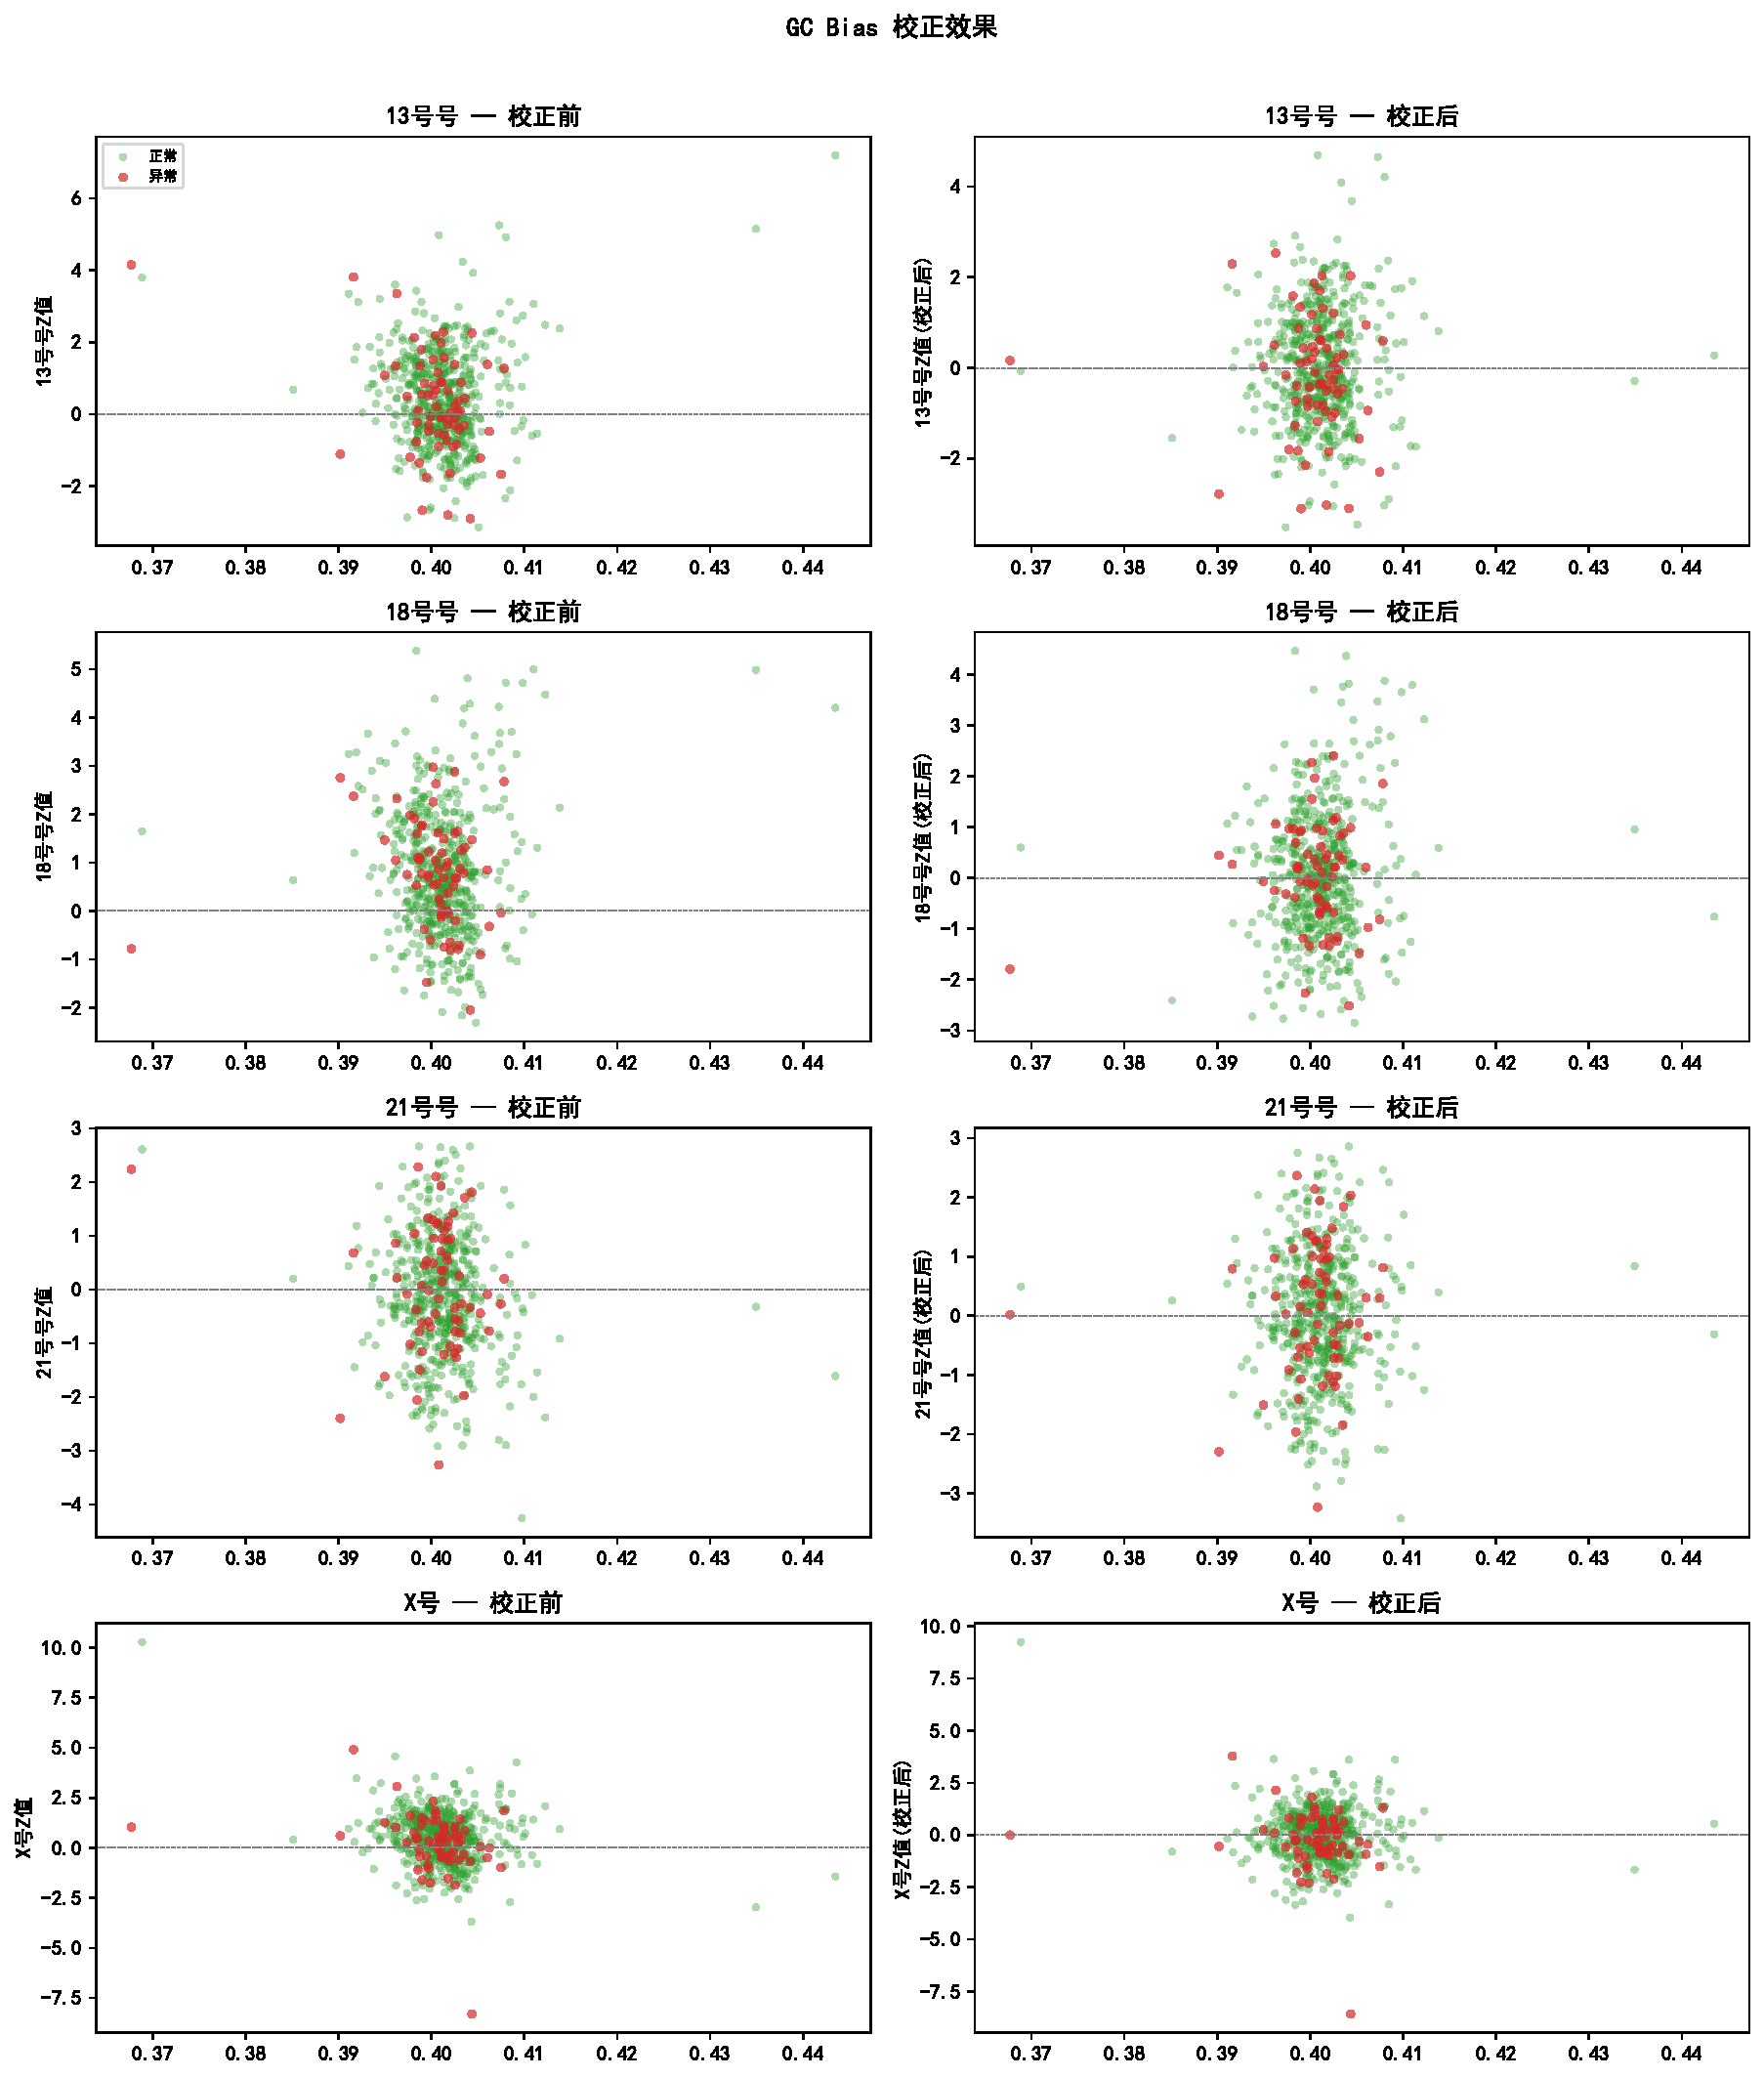
\includegraphics[width=0.55\textwidth]{sub4-gc-correction.pdf}
\caption{GC Bias 校正效果}
\label{fig:gc}
\end{figure}

\textbf{第二层——特征筛选}：单特征 Cohen's $d$ 效应量分析（表~\ref{tab:feature}）揭示：\textbf{判别力最强的并非 Z 值，而是 GC 跨染色体差异（$|d|=1.44$）和测序质控指标}。特征工程构造染色体对比值、GC 跨染色体差异、交互项。GC$_{18}-$GC$_{13}$ 与 Z18 几乎零相关（$r=0.078$），构成独立信息通道。

\begin{table}[H]
\centering
\caption{单特征判别能力排序（$|d|>0.5$）}
\label{tab:feature}
\begin{tabular}{lrrl}
\toprule
特征 & $|d|$ & $p$ 值 & 方向 \\
\midrule
18号GC$-$13号GC & 1.44 & $<0.001$ & T18 偏低 \\
X 染色体浓度    & 1.30 & $<0.001$ & 异常偏低 \\
被过滤读段比例  & 0.92 & 0.003  & 异常偏高 \\
13号GC 含量    & 0.91 & 0.004  & 异常偏高 \\
18号GC 含量    & 0.73 & 0.015  & 异常偏高 \\
孕周            & 0.77 & 0.021  & 异常偏高 \\
\bottomrule
\multicolumn{4}{l}{\footnotesize 全体 Z 值特征 $|d|<0.23$，$p>0.05$。} \\
\end{tabular}
\end{table}

\textbf{第三层——按染色体拆分 Fisher LDA + 高灵敏度阈值}：为每条染色体 $k\in\{13,18,21\}$ 单独训练判别器 $\mathbf{w}^{(k)} = (\mathbf{S}_W^{(k)})^{-1} (\boldsymbol{\mu}_1^{(k)}-\boldsymbol{\mu}_0)$，采用 Tikhonov 正则化（$\lambda=0.01\cdot\mathrm{tr}(\mathbf{S}_W)/d$）保证类内散度矩阵可逆。综合评分 $S=\max(s_{13},s_{18},s_{21})$，高灵敏度阈值 $\tau^* = \arg\min_{\tau}\{\tau:\text{TPR}(\tau)\geq 0.90\}$。并行 OR 规则初筛（过滤率、重复率、GC 含量等指标超正常组 95 分位触发），再经 Fisher LDA 精细判定。

\subsection{实验结果}

\begin{table}[H]
\centering
\caption{各策略性能对比（147 人）}
\label{tab:perf}
\begin{tabular}{lcccc}
\toprule
策略 & 召回率 & 特异度 & 漏检数 & AUC \\
\midrule
Fisher LDA (Youden)       & 81.2\% & 66.4\% & 3 & 0.775 \\
Fisher LDA (TPR$\geq$90\%) & \textbf{93.8\%} & 26.7\% & \textbf{1} & 0.775 \\
OR 规则 (K=1)             & 75.0\% & 66.7\% & 3 & — \\
Z$>3$ 基准规则            & 4.5\% & 92.6\% & 64/67 & — \\
\bottomrule
\end{tabular}
\end{table}

高灵敏度策略召回率 93.8\%（AUC=0.775），仅漏检 1 人，低风险组（26 人）安全性 96.2\%。按异常类型：T18 组 6/10 检出（信号来自 GC 差异 + X 浓度），T13 组 4/5 检出，T21 组 1/1 检出。41 条 Z 值异常但无标注样本中 37 条被标记为有风险。

\begin{figure}[H]
\centering
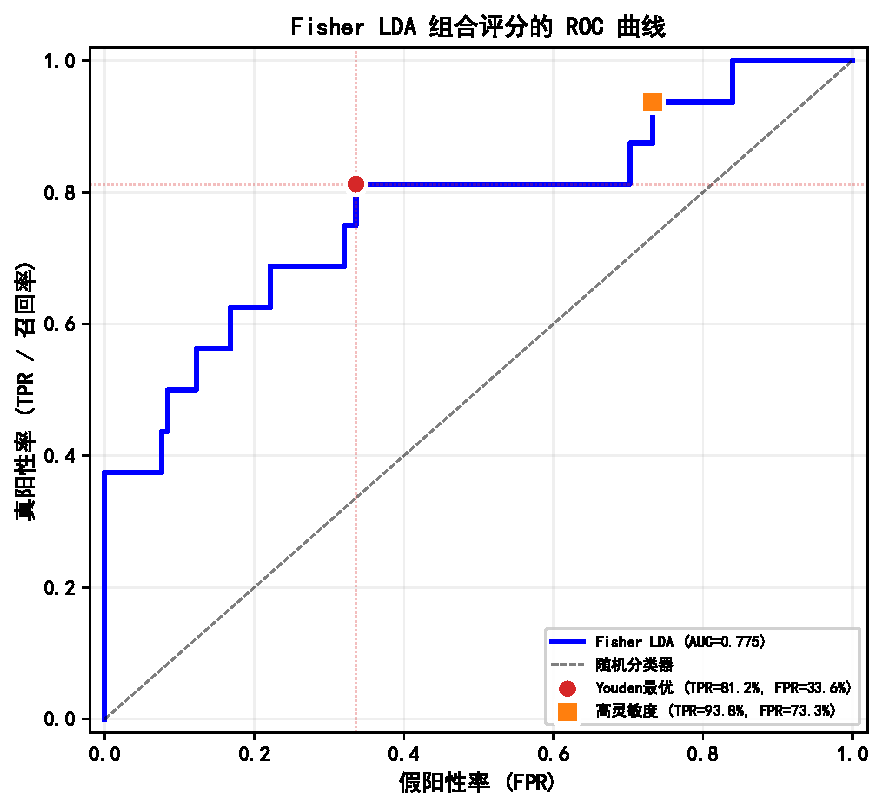
\includegraphics[width=0.5\textwidth]{sub4-roc-curve.pdf}
\caption{Fisher LDA 的 ROC 曲线（AUC=0.775）。红点=Youden，橙方块=高灵敏度。}
\label{fig:roc}
\end{figure}

\textbf{主要局限}：标注异常仅 12 人，无法实施交叉验证；T18 组 4 人漏检；约 73\% 正常孕妇被标记（筛查警戒性设计的固有代价）；GC 信号需更大规模独立验证。本方法为筛查工具（非确诊），核心创新在于发现测序质控指标和 GC 差异可构成独立于 Z 值的异常信号维度。

\newpage

% ============================================================
% 7. CONCLUSION
% ============================================================
\section{结论}

本文围绕 NIPT 的时点选择和异常判定两个核心问题，产出四项可量化结论：

\textbf{子问题 1} 揭示了纵向数据中个体基线差异的主导地位（占总变异 65\%），通过个体内中心化回归确认孕周效应（每周 $+5.7\%$，$p<0.001$）和 BMI 负效应（$-3\%$/单位，$p<0.001$）。中介分析表明 21\% 的孕周效应经 X 染色体浓度间接实现。CV $R^2=0.248$ 的诚实报告引导了后续直接计数法的保守选择。

\textbf{子问题 2 和 3} 基于非对称代价逻辑，给出按 BMI 的三级分组方案：$[28,36)$ 组 11--12 周单检（失败率 $\leq 1\%$），$[36,40)$ 组 14 周首检（失败率 8.3\%），$40+$ 组两阶段策略。多因素回归穷举检验排除 BMI 以外所有因素。$p_0$ 灵敏度和 Wilson CI 验证方案稳健，检测误差不改变分组。

\textbf{子问题 4} 在 Z 值信号缺位下构建了 GC 校正 $\to$ 按染色体拆分 Fisher LDA $\to$ 高灵敏度阈值的三层体系，召回率 93.8\%（AUC=0.775），仅漏检 1 人。核心判别力来自测序质控指标和 GC 跨染色体差异（$|d|=1.44$），而非传统 Z 值。

三项核心方法论贡献：(1) 个体基线主导地位——65\% 变异来自不可观测基线，群体回归本质失效；(2) 直接计数替代参数外推——CV $R^2=0.248$ 时拒绝将不确定性传递到临床建议；(3) Z 值缺位时发现 GC 差异和质控指标构成独立异常信号维度。

主要局限：高灵敏度策略仍漏检 1 人（现有特征空间无可识别信号）；极端样本稀疏（$[20,28)$ 仅 19 条、$40+$ 仅 18 条、标注异常仅 12 人）；子问题 4 无法交叉验证；GC 信号机制待独立验证。核心发现与文献一致\cite{wang2013,grati2014,lo1997}。

本工作以最大诚实度呈现模型预测能力边界。那个在低风险组中被漏检的 1 位患者，是对所有读者的诚实交代，也是现有数据约束下无法逾越的边界。

% ============================================================
% REFERENCES
% ============================================================
\printbibliography[heading=bibintoc,title={参考文献}]

% ============================================================
% APPENDIX
% ============================================================
\appendix
\section{补充图表}

\begin{figure}[H]
\centering
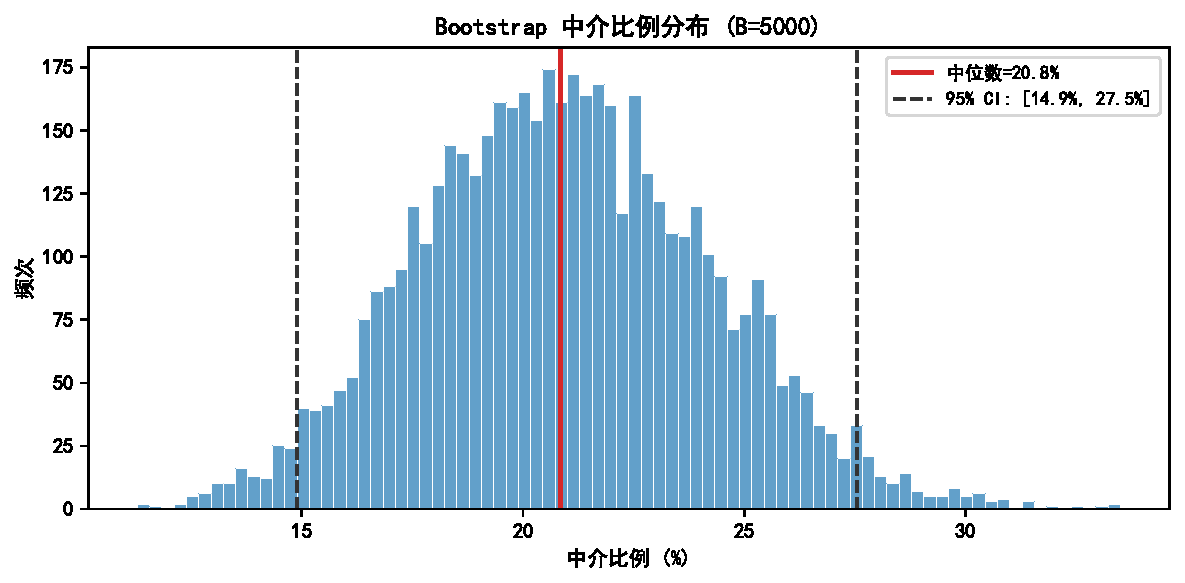
\includegraphics[width=0.55\textwidth]{sub1-mediation-bootstrap.pdf}
\caption{中介比例 Bootstrap 分布（$B=1000$）。95\% CI $[14.9\%, 27.3\%]$。}
\label{fig:boot}
\end{figure}

\begin{figure}[H]
\centering
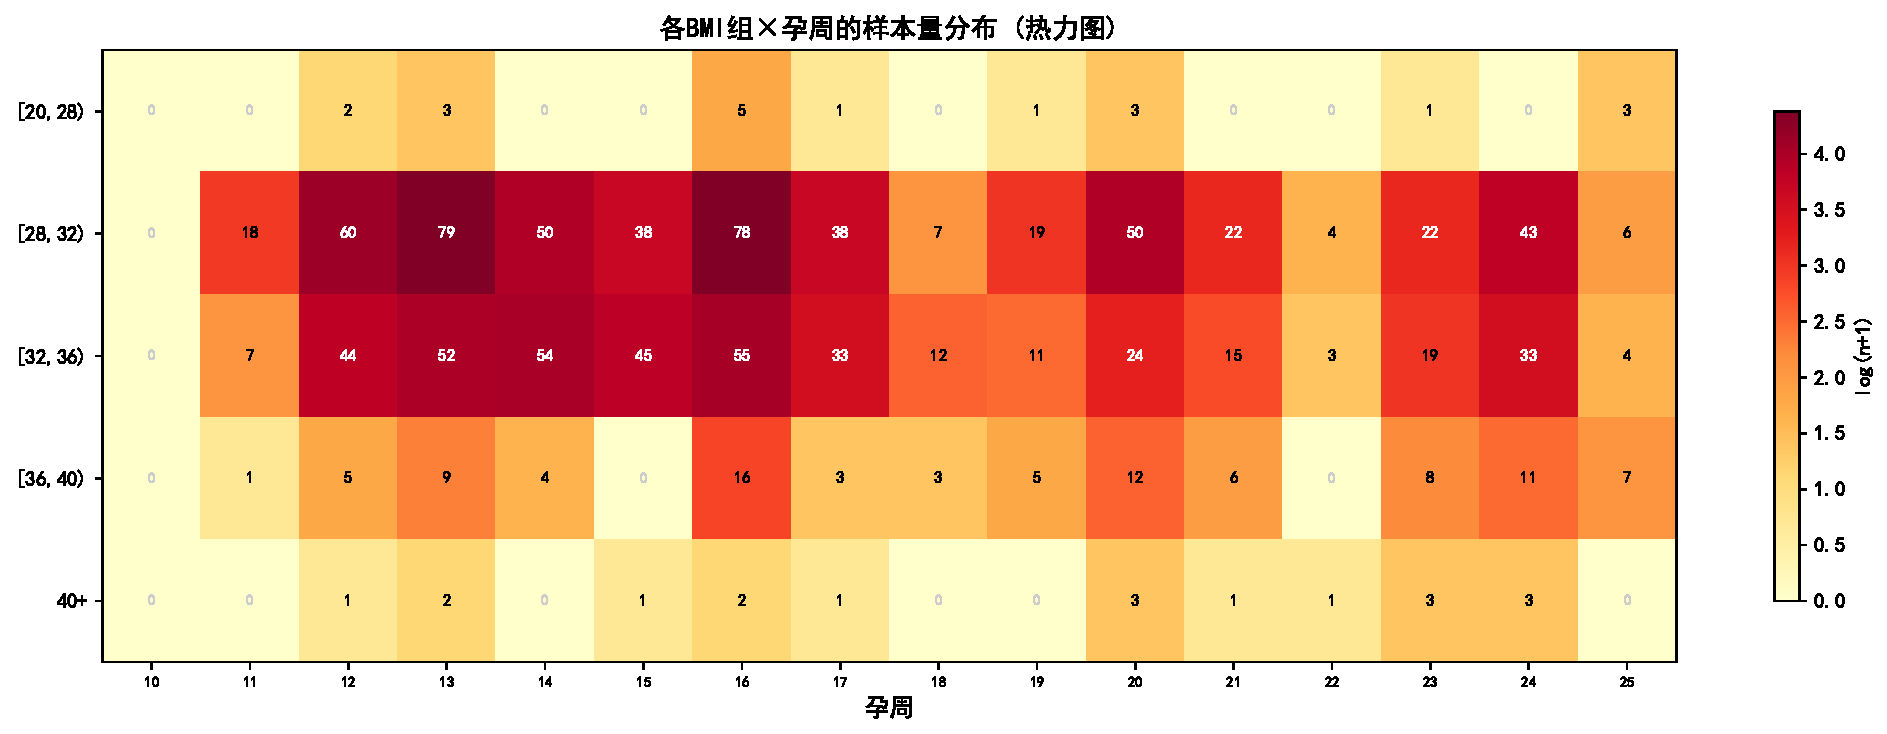
\includegraphics[width=0.7\textwidth]{sub2-cell-sizes-heatmap.pdf}
\caption{各组样本量热力图。深色=统计基础薄弱。}
\label{fig:cells}
\end{figure}

\begin{figure}[H]
\centering
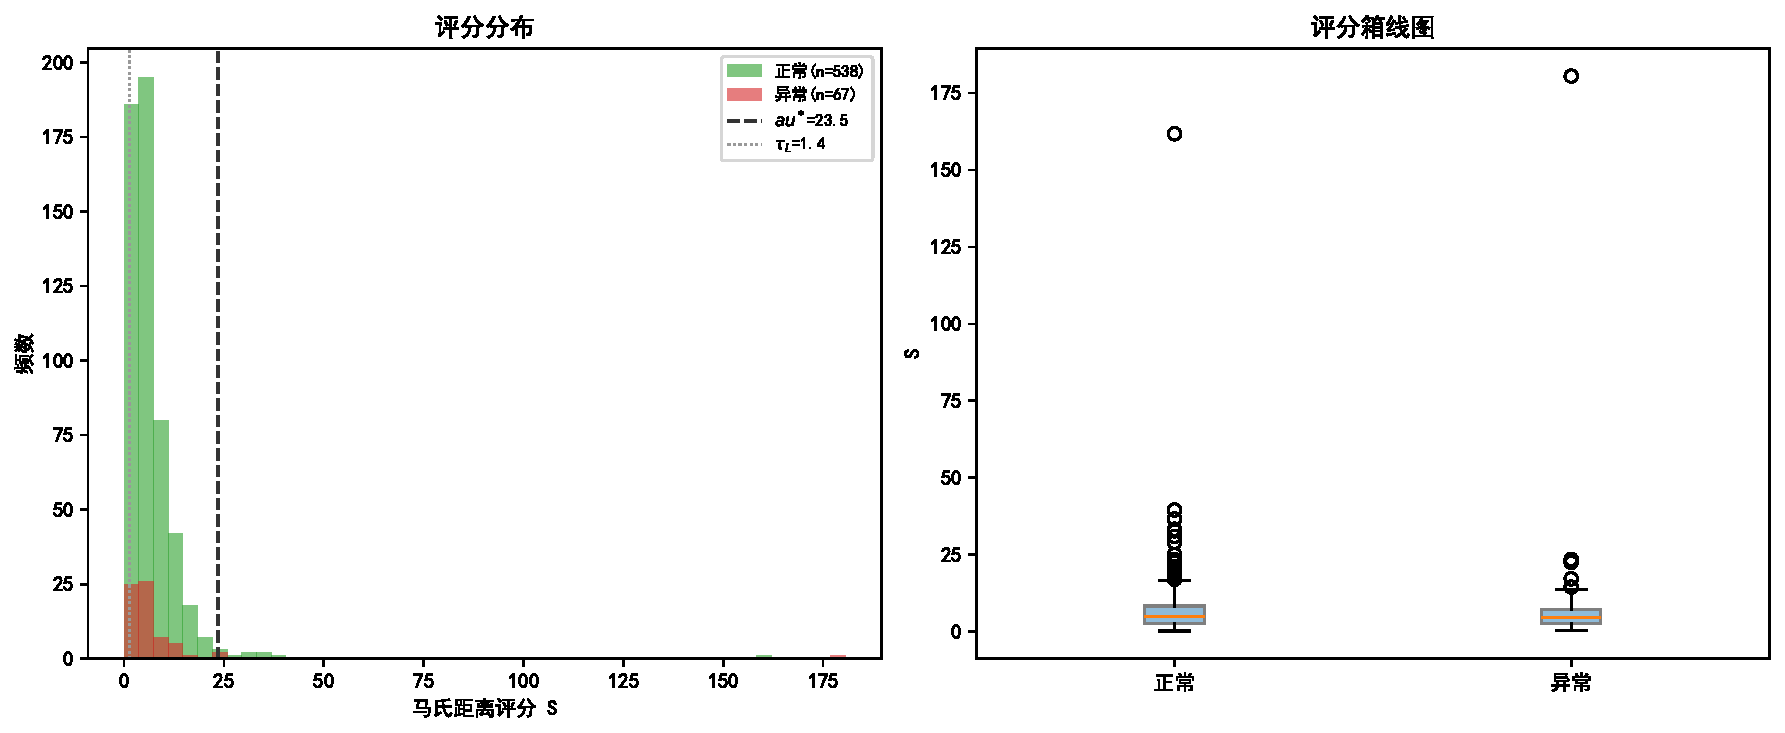
\includegraphics[width=0.55\textwidth]{sub4-score-distribution.pdf}
\caption{Fisher LDA 判别分数分布。虚线=Youden，点划线=高灵敏度。}
\label{fig:scores}
\end{figure}

\section{核心代码}

{\footnotesize
\subsection{个体内中心化回归}
\begin{verbatim}
gw_centered = df['gw'] - df.groupby('id')['gw'].transform('mean')
X = np.column_stack([gw_centered, bmi_centered, tech_features, month_dummies])
model = sm.OLS(np.log(df['y']), sm.add_constant(X)).fit()
cv_r2 = leave_one_pregnant_out_cv(model, df)  # CV R^2 = 0.248
\end{verbatim}

\subsection{Fisher LDA（Tikhonov 正则化）}
\begin{verbatim}
def fisher_lda_fit(X, y):
    X0, X1 = X[y==0], X[y==1]
    mu0, mu1 = X0.mean(0), X1.mean(0)
    S0, S1 = np.cov(X0, rowvar=False), np.cov(X1, rowvar=False)
    Sw = ((len(X0)-1)*S0 + (len(X1)-1)*S1) / (len(X)-2)
    reg = 0.01 * np.trace(Sw) / Sw.shape[0]
    w = np.linalg.inv(Sw + reg*np.eye(d)) @ (mu1 - mu0)
    return w  # w_13, w_18, w_21
\end{verbatim}

\subsection{高灵敏度阈值}
\begin{verbatim}
fpr, tpr, thresholds = roc_curve(y_true, scores)
tau_hi = thresholds[np.where(tpr >= 0.90)[0][0]]  # TPR=93.8%
\end{verbatim}
}

\end{document}
